
% This LaTeX was auto-generated from MATLAB code.
% To make changes, update the MATLAB code and republish this document.

\documentclass{article}
\usepackage{graphicx}
\usepackage{color}

\sloppy
\definecolor{lightgray}{gray}{0.5}
\setlength{\parindent}{0pt}

\begin{document}

    
    \begin{verbatim}
clear;clc

A = [0 1 0 0; 0 0 1 0; 0 0 0 1; -650 -180 -90 -6];
B = [0; 0; 0; 1];
C = [90 15 10 0];

x0 = [2; 1; 3; 0];

Ts = 2;
Mos = 2;

Mlog2 = log(Mos/100)^2;
zeta = sqrt(Mlog2/(Mlog2 + pi^2));
omegaN = 4/(Ts*zeta);

p1 = -zeta*omegaN + 1i*omegaN*sqrt(1-zeta^2);
p2 = -zeta*omegaN - 1i*omegaN*sqrt(1-zeta^2);

P = [p1 p2 -2 -7];
K = place(A,B,P)

Acs = A - B*K;
sys_o = ss(A,B,C,0);
sys_cs = ss(Acs,B,C,0);

t = 0:0.01:10;
u = ones(1,length(t));

figure, hold on
lsim(sys_o,u,t,x0)
lsim(sys_cs,u,t,x0)
grid on
title('State-feedback design')
legend('Open-loop','Closed-loop')
print(gcf,'fig3.png','-dpng','-r500');
\end{verbatim}

        \color{lightgray} \begin{verbatim}
K =

 -557.8852  -64.7834  -33.4204    7.0000

\end{verbatim} \color{black}
    
\includegraphics [width=4in]{hw82_01.eps}



\end{document}

